\documentclass[withindex, glossary]{cam-thesis}
\pdfminorversion=7

\usepackage[spanish]{babel}
\usepackage[utf8]{inputenc}
\usepackage[T1]{fontenc}
\usepackage[table]{xcolor}
\usepackage{multirow}
\usepackage{tabularx}
\usepackage{graphicx}
\usepackage{lmodern}
\usepackage{cleveref}

\usepackage{hyperref}
\addto\extrasspanish{%
    \def\chapterautorefname{capítulo}%
}

\usepackage{svg}
\usepackage{multicol}
\usepackage{mathtools}
\usepackage{booktabs}
\usepackage{bookmark}
\usepackage{blkarray, bigstrut}
%\usepackage{subcaption}
\usepackage{pgfgantt}
\usepackage{array}
\usepackage[capposition=top]{floatrow}

\usepackage[backend=biber, style=ieee, sorting=ynt]{biblatex}
\addbibresource{thesis.bib}

\usepackage{minted}
\usemintedstyle{manni}

\usepackage{csquotes}

\usepackage{tikz}
\usetikzlibrary{shapes.geometric, arrows.meta, fit, backgrounds, positioning, matrix, decorations.pathreplacing, calc}
\tikzstyle{startstop} = [rectangle, rounded corners, minimum width=3cm, minimum height=1cm,text centered, draw=black, fill=red!50]
\tikzstyle{io} = [trapezium, trapezium left angle=70, trapezium right angle=110, minimum width=3cm, minimum height=1cm, text centered, draw=black, fill=blue!30]
\tikzstyle{process} = [rectangle, minimum width=3cm, minimum height=1cm, text centered, draw=black, fill=orange!30]
\tikzstyle{decision} = [diamond, minimum width=3cm, minimum height=1cm, text centered, draw=black, fill=green!20]
\tikzstyle{database} = [cylinder, minimum width=3cm, minimum height=2cm, text centered, shape border rotate=90, aspect=0.25, draw=black, fill=yellow!30]
\tikzstyle{arrow} = [thick, ->, >=stealth]
\tikzstyle{line} = [-Latex]
\newcommand{\inline}[2]{%
    \begin{tikzpicture}[baseline=(word.base), txt/.style={shape=rectangle, inner sep=0pt}]
        \node[txt] (word) {\texttt{#1}};
        \node[above] at (word.north) {\footnotesize{#2}};
    \end{tikzpicture}%
}

\usepackage{pgfplots}
\pgfplotsset{compat=newest}

\setlength{\columnseprule}{0.4pt}

\title{Máster en Computación Gráfica y Simulación\protect\\\bigskip \normalfont{2018\protect\\\bigskip Trabajo Final de Máster\protect\\\bigskip Estudio sobre sistemas de anti-aliasing e implementación de anti-aliasing temporal}}
\author{Hugo Ferrando Seage}
\submissiondate{Tutor: Dr.~Alberto Sánchez Campos}

% PDF meta-info
\subjectline{Máster en Computación Gráfica y Simulación}
% max 6
\keywords{opengl antialiasing temporal}

% Abstract
\espabstract{%
    Debido a la resolución limitada de las pantallas al \gls{rasterizar} gráficos 3D se deforman ciertas lineas y curvas. Este fenómeno se llama aliasing. La demanda de gráficos cada vez más realistas ha propiciado la creación de diferentes técnicas y algoritmos para disimular estos defectos, sin tener que recurrir necesariemente a pantallas de mayor resolución.

    El antialiasing se ha vuelto una técnica crucial para mejorar la calidad de imagen en el software con gráficos tridimensionales. Este campo de la computación gráfica lleva años desarrollandose, con nuevas técnicas publicadas continuamente.

    Este proyecto tiene como objetivo el análisis de las distintas técnicas existentes en el estado del arte y la implementación de un algoritmo de temporal antialiasing, compatible con motores con deferred shading y comparable en calidad al multisampling, junto a otras propiedades.
}

\abstract{%
    When rasterizing 3D graphics using computer screens, due to their limited resolution some lines and curves will become deformed. This phenomena is called aliasing. The ever increasing demand for more realistic graphics has driven the creation of new techniques and algorithms to hide these artifacts, without necessarily using higher resolution screens.

    Antialiasing has become a crucial technique to advance image quality in graphics software. This field has been explored for years, with new approaches being developed continually.

    This projects aims to analyze different antialiasing techniques developed and the implementation of a temporal antialiasing technique, compatible with deferred shading engines and with similar quality to mutlisampling, amongst other benefits.
}

% Glossary
\newglossaryentry{rasterizar}{%
    name=rasterizar,
    description={Conversión de una imagen descrita con alguna primitiva (curvas, vectores, triangulos) a un conjunto de pixels}
}

\newglossaryentry{opengl}{%
    name=OpenGL,
    description={API estándar para el desarollo de software con gráficos 2D o 3D con aceleración por hardware\cite{Kessenich:2016:OPG:3013620}}
}

% Acronyms

% Contents
\begin{document}
\frontmatter{}

% Thesis body:
\chapter{Introducción}
\section{¿Qué es el aliasing?}

El antialiasing es la deformación de ciertos elementos gráficos al ser rasterizados y plasmados en una pantalla con una resolución finita\cite{Mitchell:1988:RFC:378456.378514}. Normalmente los bordes de la geometría que tengan ángulos que no se alineen perfectamente con los pixels presentaran bordes de sierra abruptos, que no es fiel a la escena como se vería de forma natural.

Este proyecto se centra en aliasing dentro del campo de la computación gráfica, pero afecta a otras disciplinas, como el procesamiento de señales (por ejemplo al digitalizar señales de audio analógicas). En general, al representar valores continuos en algún medio discreto siempre habrá algún defecto de este tipo\cite{Mitchell:1988:RFC:378456.378514}.

Existen otros tipos de aliasing, como en el interior de texturas o al mover la camera rápidamente.

\section{¿Qué es el antialiasing?}

El antialiasing es el conjunto de técnicas cuyo objetivo es el de disimular o eliminar estas imperfecciones.

\chapter{Planteamiento del problema}

El aliasing siempre ha sido un problema en el campo de la computación gráfica. Desde la década de los 70 se han usado técnicas como la interpolación bicubica para el renderizado de imagenes por ordenador con ray-tracing.

Durante la década de los 80 y buena parte de los 90 hubo un avance constante en términos de potenica, resolución y la capcidad de mostrar cada vez más colores (por ejemplo del paso de gráficos CGA a VGA). Aún así el rendimiento necesario para aplicar muchas de las técnicas de antialiasing solo se podian usar con workstations profesionales, como las IRIS de Silicon Graphics.

A mediados de los 90, con la llegada de la tarjetas aceleradores de gráficos 3D a ordenadores mas modestos las compañías como ATI, NVIDIA y 3DFX empezaron a integrar soluciones de antialiasing a sus productos y APIs.

A la vez que evolucionaba el hardware los gráficos cada vez requerian más potencia. Las técnicas como el supersampling reducen drásticamente el rendimiento, por lo que en muchos casos se empezaron a usar optimizaciones como el multisampling.

Con la llegada de los shaders programables y el deferred shading el multisampling empezó a no poder ser usado en muchos casos. Por ello se desarrollaron algoritmos como el MLAA, FXAA y SMAA que son compatibles tanto con el forward shading como el deferred shading y con un impacto muy bajo en el rendimiento.

Al contrario que el supersampling, el multisampling y el post-processing antialiasing no solucionan todos los tipos de aliasing que tiene una imagen. Para intentar aunar las ventajas del supersampling con el rendimiento y compatibilidad del post-processing antialiasing se han empezado a desarrollar técnicas de antialiasing temporal, como el TXAA.

\chapter{Objetivos}

Este proyecto tiene dos objetivos principales:

\begin{enumerate}
    \item Analizar el estado del arte en el campo de la computación gráfica en relación al anti-aliasing. Explorar los problemas que presenta el aliasing en gráficos 2D y 3D, la evolución de las soluciones y los desarrollos en curso.
    \item El segundo objetivo es el de integrar una solución de anti-aliasing temporal a un motor gráfico 3D existente desarrollado durante la asignatura de APIs tridimensionales del Máster en Computación Gráfica y Simulación cursado.
\end{enumerate}

\chapter{Estado del Arte}

\section{Aliasing en bordes de geometría}

Cuando se piensa en los defectos del aliasing lo primero que viene a la cabeza es este tipo de defecto. Al rasterizar los polígonos, los bordes de la geometría no se ven con una línea suave, si no que tienen un único color y tienen una forma de escalón.

imagen

\section{Aliasing de texturas}

Dentro de las texturas tambien puede haber aliasing. Al igual que pasa en los bordes de la geometría, al cambiar de un color a otro rápidamente se pueden ver esos mismos defectos. Si una textura contiene alguna linea que no se alínee correctamente con la pantalla tambien se pueden apreciar estos defectos.

Posibles soluciones: Mip Maps, LoD

\section{Specular Aliasing}

La iluminación especular es aquella 
Durante el calculo de la iluminación especular que se refleja en los materiales como el metal o el plástico a veces

\section{Motion Aliasing}

A veces al mover la cámara tambien se pueden producir efectos de aliasing. El efecto no se puede apreciar en una imagen fija, pero al verlo el movimiento es un efecto que distrae. Recuerda al parpadeo de una luz, que una vez que la cámara permancece quieta desaparece.

Este tipo de aliasing se suele solucionar con técnicas de blurring, que recuerdan más al efecto del cine a 24FPS que a técnicas de antialiasing como las que se explican a continuación.

A veces tambien se conoce como crawling.

Conforme el hardware ha ido evolucionando durante los años, tambien lo han hecho las técnicas empleadas para simular el efecto de blurring de las cámaras con la intención de hacerlo más realista.

Explicar motion blur en cámaras

Las cámaras de video capturán la luz durante un breve periodo de timepo para capturar cada isntantanea usada en un video. 

Una de las primeras técnicas era la de usar un buffer de acumulación, combinarlo con el frame n y ir actualizandolo con n frames. La desventaja de este efecto es que emborrona toda la escena por igual y puede resultar incluso más desagradable que el propio aliasing.

Con la llegada de los shaders se empezaró a usar per pixel motion blur. Para esto hace falta calcular donde estaba cada pixel en el frame n-1 y simular algun efecto con esa información.

El per object motion blur es un refinamiento de la anterior, donde en vez de calcular donde estaba cada pixel en el frame anterior, haces el cálculo por cada poligono de la escena. Eso significa que es posible añadir más blurring a algún objeto y dejar el resto de la escena con mayor detalle.

\section{Filtrado}
\label{filtros}

En gráficos raster (bidimensionales) el anti-aliasing se realiza mediante filtros.Para entender el filtrado en imágenes es necesario pensar en pixels no como pequeños cuadrados en una pantalla, si no en muestras de una función (normalmente 3 muestras, una por cada canal RGB)\cite{Smith95apixel}. Los filtros (o kernels) transforman las funciones para intentar suavizar los cambios bruscos de color.

En la figura~\ref{gls} se muestra una comparación de las diferentes formas en las que cada filtro interpola valores de una imagen con un solo canal. Cada punto representa la muestra de la función que se visualizará en la pantalla.

%\cite{resampling}

\begin{figure}[!htb]
    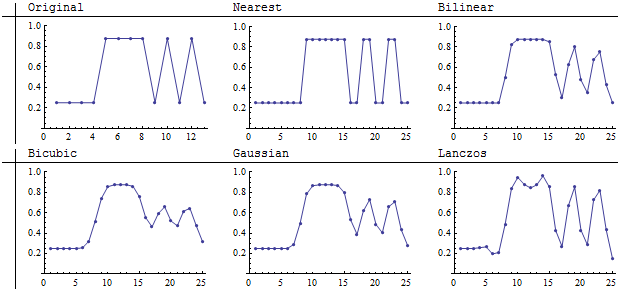
\includegraphics[width=\linewidth]{figures/Lw6ei.png}
    \caption{Comparación de interpolación usando diferentes filtros\cite{gis}}
    \label{gls}
\end{figure}

\begin{figure}[!htb]
    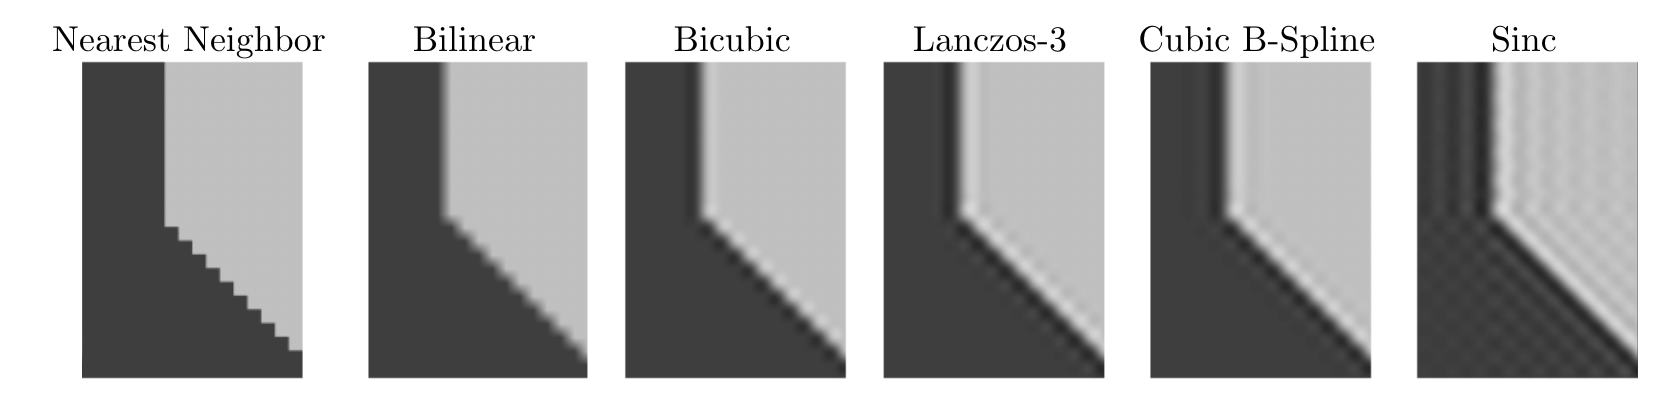
\includegraphics[width=\linewidth]{figures/comparison-filter.png}
    \caption{Comparación de resultados de diferentes filtros\cite{resampling2}}
\end{figure}

\section{Supersampling Antialiasing}

El supersampling consiste en minimizar el aliasing usando imágenes con una resolución mayor a la usada para su visualización (antialiasing espacial). Cada pixel en la pantalla será representado por más de un pixel en la imagen. Para el color final normalmente se hace la media del valor de los colores de los múltiples pixels.

Estas técnicas consumen más ancho de banda y memoria, ya que los buffers tienen que guardar más información por pixel que la imagen original.

La calidad del supersampling viene dado por la cantidad de samples por pixel y la técnica para saber que pixels usar en la imagen con mayor resolución para cada pixel de la pantalla.

En comparación a otras técnicas de antialiasing esta corrige aliasing de texturas y especular, además de aliasing de geometría. Esto se debe a que los subsamples los coge de en toda la escena.

\subsection{Ordered Grid Supersampling}

En esta técnica de supersampling la distribución de los samples es uniforme. Debido a la naturaleza regular de este patrón, los subpixels se encuentran situados en forma de dos columnas y dos filas. Para lineas muy planas, tanto en horizontal como vertical el antialiasing no será muy efectivo, ya que muy rápidamente tocará dos subpixels en fila o columna y hasta el final no tocará los otros subpixels, como se puede ver en la figura~\ref{ogss}.

Este efecto se puede reducir usando más samples, pero el impacto en el rendimiento será todavía mayor.

Desde 2014 Nvidia ha publicado una técnica llamada Dynamic Super Resolution\cite{960}, que consiste en renderizar software a mayor resolución y usar OGSS con un filtro de blur gaussiano. En 2015 AMD implementó una técnica similar llamada Virtual Super Resolution.

\begin{figure}[!htb]
    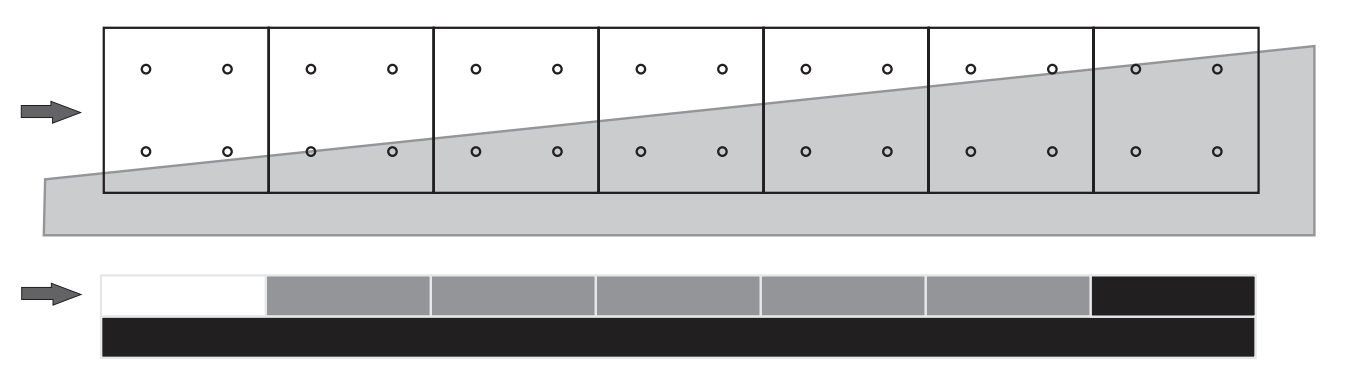
\includegraphics[width=\linewidth]{figures/ogss.png}
    \caption{Ordered Grid Super-Sampling\cite{Beets2000SupersamplingAA}}
    \label{ogss}
\end{figure}

\subsection{Rotated Grid Supersampling}

Aquí la idea es cambiar el lugar de los subsamples para minimizar la cantidad de columnas y filas. La distribución sigue siendo uniforme, pero el problema del aliasing en lineas muy planas se soluciona, como se puede apreciar en la figura~\ref{rgss}, sin tener que recurrir a aumentar de manera significativa el numero de subsamples.

\begin{figure}[!htb]
    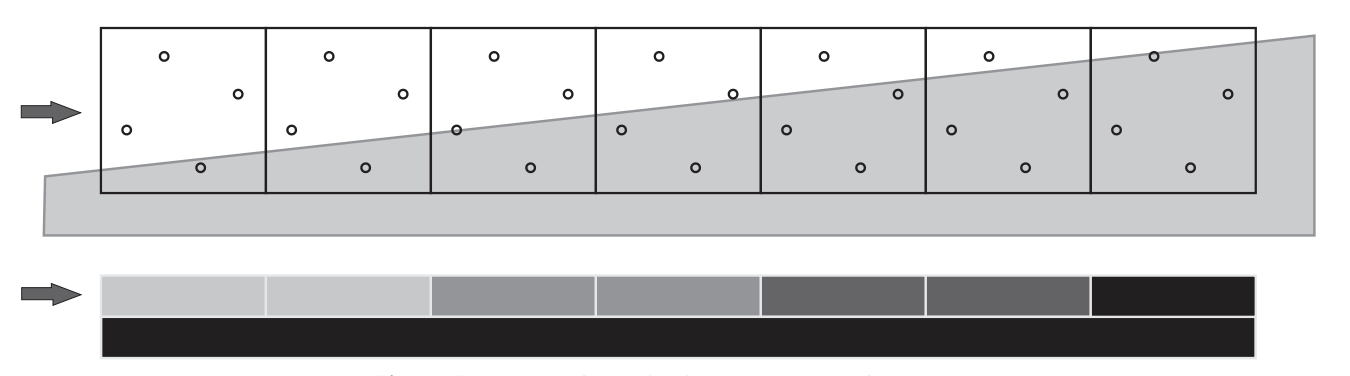
\includegraphics[width=\linewidth]{figures/rgss.png}
    \caption{Rotated Grid Super-Sampling\cite{Beets2000SupersamplingAA}}
    \label{rgss}
\end{figure}

\subsection{Quincunx Supersampling}

Este patrón es interesante como técnica de supersampling ya que usa subsamples localizados en las esquinas de los pixels, lo que permite reutilizar varios subsamples entre pixels (figura~\ref{fig:quincunx}). Esto permite una calidad similar a la de un antialiasing 4x pero con un coste computacional de un supersampling 2x. Aún así al reutilizar subsamples produce resultados algo más borrosos que otros métodos.

Aunque este patrón se pueda usar para supersampling Nvidia lo implementó en hardware desde la GeForce 3\cite{hraa} para acelerar el calculo de su multisampling. Sony al utilizar una GPU de Nvidia en la PS3 también disponía de esta tecnología en la consola.

\begin{figure}[!htb]
    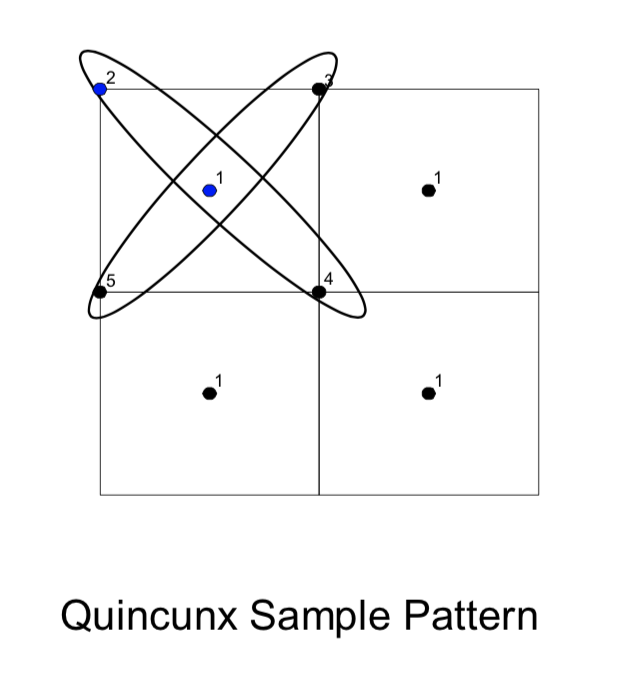
\includegraphics[width=\linewidth]{figures/quincunx.png}
    \caption{Quincunx Pattern\cite{hraa}}
    \label{fig:quincunx}
\end{figure}

\section{Multisampling}

Multisampling es una optimización del supersampling. Se sigue usando subpixels, pero en vez de resolver el color para cada subpixel el color se resuelve una única vez por pixel. Después de resolver el color se calcula el stencil buffer y depth buffer con subpixels, y dependiendo de la cantidad de subpixels que estén contenidos dentro del triangulo se usará un porcentaje del valor del color calculado. Esto reduce drásticamente el impacto en el rendimiento de la aplicación, ya que solo hay que acceder una vez por pixel a la textura, pero solo soluciona aliasing en los bordes de la geometría.

En el centro de un polígono todos los subpixels van a estar contenidos dentro, pero el color solo se calcula una vez (por ejemplo en el centro del pixel), por lo que se usará el 100\% del color, pero puede contener aliasing. En cambio, en los bordes, algún subpixel estará fuera de la geometría, por lo que se usará un porcentaje del color calculado, suavizando el borde.

Otra de las desventajas del multisampling anti-aliasing es que, tradicionalmente, no se puede usar en motores con deferred shading. Debido a que el calculo del color final de cada pixel se realiza en un pixel shader posterior al calculo del g-buffer, al hacer el resolve del mutisampling no esta lista toda la información necesaria. Desde OpenGL 3.2 y Direct3D 10.1 esto ha cambiado gracias al explicit multisampling\cite{textureMultisample}. La creación del g-buffer ahora se puede realizar usando texturas multisampled y al calcular la luz se puede acceder a los subsamples mediante la función texelfetch. Si se realiza de esta forma hay que sacrificar la creación automática de mipmaps y filtrado de texturas, aunque siempre se pueden implementar manualmente en shaders. Aún así muchos desarrolladores han optado por usar post-processing antialiasing al usar deferred shading.

\section{Post Processing Antialiasing}

Este tipo de antialiasing ha ganado popularidad durante los últimos años, debido en parte al uso del deferred shading en los últimos motores gráficos. Los algoritmos presentados a continuación se pueden considerar filtros de rasters, como los de la sección~\ref{filtros}, pero están pensados para ser usados en motores gráficos. Además, en muchos casos, usan información que no esta presente en la textura final, como pueden ser texturas de profundidad o vectores de movimiento,

\subsection{Fast Approximate Anti-aliasing}

El FXAA\cite{FXAA} es un sistema de anti-aliasing de post procesado desarrollado por NVIDIA\@.

\subsection{Morphological Antialiasing}
mlaa

\subsubsection{Enhanced Subpixel Morphological Antialiasing}
smaa

\subsection{Temporal Antialiasing}

El temporal antialiasing es un tipo de antialiasing de post procesado, pero que amortiza el coste computacional usando múltiples samples en múltiples frames. Esto presenta unas complicaciones a la hora de escoger samples en frames anteriores en imágenes no estáticas.

\chapter{Desarrollo}

Para este proyecto se ha integrado un sistema de anti-aliasing temporal en un motor de gráficos 3D que usa \Gls{opengl} como API gráfica.

\section{History Buffer}

Debido a la necesidad de combinar varias texturas de frames anteriores, para computar el anti-aliasing de un frame n es necesario tener acceso al frame n-1. Aún usando más de 2 subsamples solo es necesario guardar el último, siempre y cuando tenga el antialiasing ya incluído.

También se puede optar por guardar n frames para n subsamples y combinarlos en un pixel shader, pero esto ocupa mucha más memoria.

\section{Jitter}

En primer lugar es necesario elegir los subsamples a usar en cada frame. Recordemos que en vez de calcular varios subsamples en cada frame, el temporal antialiasing calcula un solo sample por frame. Cada frame cambiará el lugar del subsample a calcular Gracias a que solo se calcula un subsample por frame el impacto en el rendimiento será mucho menor al del supersampling tradicional.

Para elegir los subsamples se pueden usar los grids vistos anteiormente en la sección sobre supersampling REF. Aún así en la práctica se suelen usar secuencias de Halton.

Las secuencias de Halton proporcionan una baja discrepancia, lo que significa que no se van crear clusters ni en espacio ni en tiempo. Esto proporciona una calidad de subsamples muy alta por lo que la calidad del antialiasing puede ser muy elevado. Siempre que esté bien implementado los resultados serán mejores que los del antialiasing por hardware implementado hasta ahora. CITAR

Una vez se ha calculado la secuencia de Halton en cada frame se alterará la matriz MVP para mover el sample al lugar del subsample que toque en ese frame. Este lugar cambiará cada vez que se genera un nuevo frame.

En este punto si viésemos la imagen seguiríamos notando el aliasing y la imagen parecería que estuviera vibrando ligeramente.

\section{Motion Vectors}

El segundo paso para la implementación del temporal anti-aliasing consiste en la creación de unvelocity buffer. Este buffer contendrá una textura con dos canales de color (rojo y verde) donde cada pixel representa un vector.

Estos vectores representan cuanto se ha movido ese pixel en el espacio de la pantalla (screen sapce) de este frame (n) al frame anterior (n-1). Con este buffer es posible combinar el history buffer que contiene el frame anterior con el antialiasing con la textura del frame del que se quiere hacer el anti-aliasing.

Cada pixel viene dado por su posición en la pantalla x e y. Al combinar texturas se combinan un pixel xy con el pixel xy - rg del history buffer (PONER ECUACIÓN).

Para la creación del velocity buffer en una escena dinámica es imprescindible saber no solo el movimiento de cámara del frame anterior, si no como se han movido los objetos. Esto se complica si hay objetos translucidos como ventanas.

En este proyecto se ha optado por usar el algoritmo descrito en (GPU GEMS CH 27) para su implementación. Solo usan pixel shaders junto al history buffer, el depth buffer y las matrices VPn y VPn-1. La ventaja de este algoritmo es que no depende mucho de la implementación del motor. Nvidia incluye una librería que hace estos calculas en el SDK NvidiaWorks (usado para la implementación de TXAA) CITAR NVIDIAWORKS.

Otra posibilidad es computar la velocidad durante una segunda pasada del vertex shader de cada polígono, pero dependiendo de su implementación puede resultar algo más lenta. Aún así debería resultar en vectores más precisos y en algunas ocasiones no queda más remedio que implementarlo así.

\section{Combinación de texturas}

\section{Neighborhood Clamping}

Los motion vectors a veces no son suficientemente precisos como para poder usarlos por si solos. Si un objeto ocluye a otro durante un cambio de frame el pixel resultante tendrá un color incorrecto, ya que se combinaran texturas de dos objetos diferentes.

Para solucionar esto se puede usar neighborhood clamping. Cada pixel se compara con el valor de los pixels adyacentes. Si el cambio de color es brusco y supera el umbral configurado se descarta la información del history buffer para ese pixel y se queda sin antialiasing hasta el siguiente frame.

EL GHOSTING TAMBIENS E PUEDE DISIMULAR USANDO BLURRING

\section{Sharpening kernel}

Debido a la naturaleza del temporal antialiasing la imagen final puede resultar demasiado suave. Los bordes quizás resulten algo difusos. Este efecto puede no ser del agrado del usuario. Una posible solución es usar un kernel de sharpening que resalta los bordes de la geometría.

\chapter{Resultados}

A continuación se encuentran algunos resultados.

\begin{figure}[!htb]
    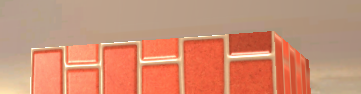
\includegraphics[width=\linewidth]{figures/taaoff.png}
    \caption{Anti-aliasing off}
    \label{aaoff}
\end{figure}

\begin{figure}[!htb]
    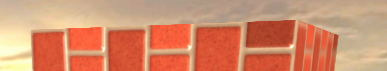
\includegraphics[width=\linewidth]{figures/taa8.png}
    \caption{Temporal anti-aliasing con 8 samples}
    \label{taa8}
\end{figure}

\begin{figure}[!htb]
    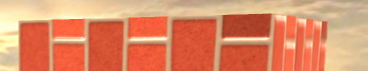
\includegraphics[width=\linewidth]{figures/taa16.png}
    \caption{Temporal anti-aliasing con 16 samples}
    \label{taa16}
\end{figure}

\chapter{Conclusión}

% Bibliography:
\nocite{*}
\printbibliography{}

\listoffigures
\listoftables

% Index
\printthesisindex{}

\end{document}
